\documentclass[a4paper, 12pt, oneside]{article}
\usepackage[utf8]{inputenc}
\usepackage[english]{babel}
\usepackage{fancyhdr}
\usepackage{geometry}
\usepackage{graphicx}
\usepackage{float}
\usepackage{subfig}
\usepackage{epstopdf}
\usepackage{amsmath}
\usepackage{amssymb}
\usepackage{siunitx}
\usepackage{enumitem}
\usepackage{booktabs}
\usepackage{gensymb}
\usepackage{makecell}
\usepackage{indentfirst}
\usepackage{bigints}
\usepackage{esint}
\usepackage{harpoon}
\usepackage{relsize}
\usepackage{CJKutf8}
\usepackage{cite}
\usepackage{url}
\usepackage{chemformula}
\usepackage{multicol}
\usepackage[useregional]{datetime2}
\usepackage[colorlinks = true,linkcolor = blue,hypertexnames = true]{hyperref}
\hypersetup{
    colorlinks=true,
    allcolors=blue	
}
\usepackage[super, square]{natbib}
\usepackage{multicol}
\usepackage{fancybox}
\usepackage{authblk}
\usepackage[many]{tcolorbox}

\newtcolorbox{fancyquotes}{%
    enhanced jigsaw, 
    breakable,      % allow page breaks
    frame hidden,   % hide the default frame
    left = 1cm,       % left margin
    right = 1cm,      % right margin
    overlay={%
        \node [scale=8,
            text=black,
            inner sep=0pt,] at ([xshift=-1cm,yshift=-1cm]frame.north west){``}; 
        \node [scale=8,
            text=black,
            inner sep=0pt,] at ([xshift=1cm]frame.south east){''};  
            },
        % paragraph skips obeyed within tcolorbox
                parbox=false,
}



\newenvironment{shadequote}%
{\begin{snugshade}\begin{quote}}
{\hfill\end{quote}\end{snugshade}}



\newcommand{\splitter}{\noindent\rule{\linewidth}{0.5pt}}

\geometry{a4paper, scale = 0.85}
\linespread{2.0}


\begin{document}
\begin{CJK}{UTF8}{bkai} % bsmi %bkai

\title{改變聽音樂的習慣}
\author[1]{張德權}
\affil[1]{Student at Department of Physics, National Taiwan University}






\date{\DTMdate{2022-08-08}}
\maketitle

\section*{串流音樂可以隨時填補生活空白}
在串流音樂在給人們帶來更快速的音樂、帶給串流平台大量收入的同時也擠壓了音樂製作人的生存空間。以 iTunes 平均一首歌 0.99 美金舉例，實際支付給歌手的利潤大約在 0.5 美金、因地區而異；但是在串流平台上則是以「播放次數」作爲支付依據，價格因平台而異，但利潤普遍無法達到曾經的數位下載；另外據估計在 Spotify 平台上「一次都沒有被播放過」的音樂大約有 400 萬首。
\begin{figure}[H]
\centering
\shadowbox{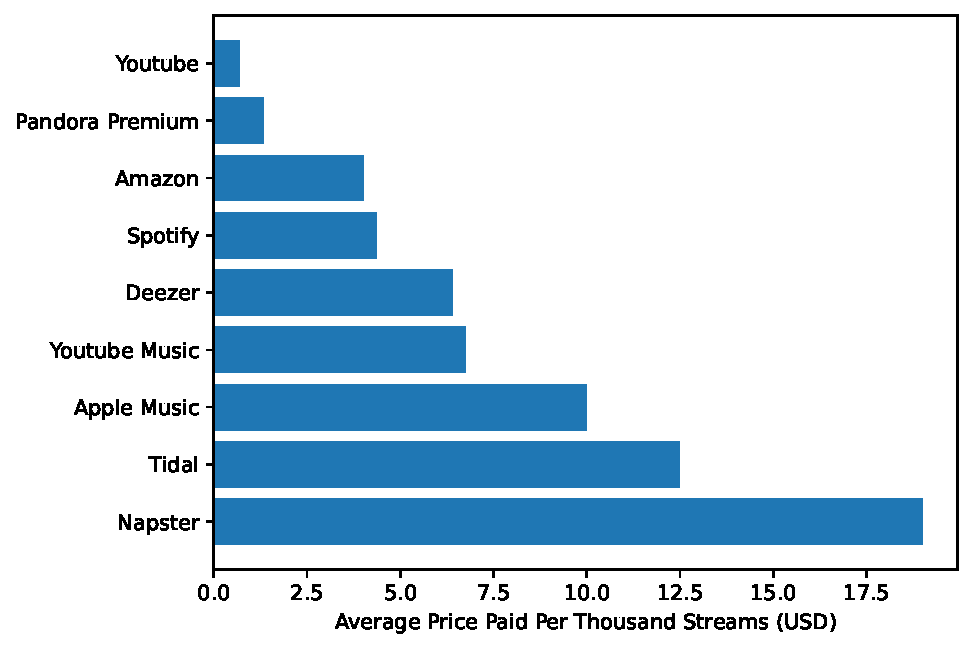
\includegraphics[width = 4in]{../Money_Too_Tight_To_Mention_2018.pdf}}
\caption{各大平台音樂播放分潤}\label{p1}
\end{figure}

稍微計算一下就會發現，你每個月一百多塊的訂閱費沒有幾塊錢真正去到了歌手那裡，大多都進入了串流平台的手上。

儘管如此，以上數字是在 Spotify 艱難獲利、Apple Music 公開調漲分潤之後的結果，對於創作者來說顯然不夠理想。因此，我推薦你暫時脫離串流平台的束腹、用傳統的方式體會音樂，邁向更健康的音樂環境。

\begin{fancyquotes}
	截至今日（2022 年 8 月 8 日），我已經從 iTunes 上購買了 513 首音樂，一共花費新台幣 10,260 元。第一次的購買日期是（2017 年 8 月 8 日）、音樂庫中最高的播放次數是 763 次。若都使用標準版的 Apple Music 則是會花費新台幣 10,800 元。對於我來說，串流音樂並沒有比較省錢。
\end{fancyquotes}
\section*{音樂載體}
2015 年 Apple 推出 Apple Music，2018 年 Spotify 在紐交所上市。不難看出串流音樂市場正在填補人們在這個忙碌的世界對音樂的需求；聽音樂的載體再一次進化了。從黑膠、卡帶、CD、數位化專輯一直到現在的串流，音樂的載體一次次的得被超越、取代。每一次的轉變都會有人不喜歡，直到今日還是會有人告訴你「黑膠聽才得出溫度」、「CD 的音質是最的」；這些理由不是空穴來風，黑膠確實能在對的流程下紀錄更多細節，CD 中動輒數百 MB 的檔案比起一首不到 20MB 的 iTunes 下載版在取樣率上有顯而易見的優勢。但這一些優勢都比不上音樂載體變的更小、更易攜帶的趨勢。勢不可擋的串流音樂必將統一江湖；但是在數位購買管道完全消失前，我們還保有選擇。
\begin{fancyquotes}
	沒人可以逆轉時代的洪流，但是保有選擇權也不是一件壞事。
\end{fancyquotes}

\section*{隨機撥放}
從數位時代開始，人們一直以來的需求：不受限制的購買單曲被滿足了。一張專輯對多數人來說總是有幾首歌很多餘，不過這種情況以 iTunes 不是個問題，畢竟購買整張專輯的價格通常小於避開那些歌並只購買單曲的價格；但當一張專輯中只喜歡其中的ㄧ、二首歌時單曲購買就是一個非常省錢的方式了。當你的音樂庫中充斥著一首首來自不同專輯的音樂時播放音樂的方式便很重要了，要是天天以字母順序播放肯定很快就膩了；因此，「隨機播放」是多數人的選擇。

以領頭羊 Spotify 來說，Spotify 能如此快速的佔領市場靠的是他的獨門絕技「讀心術」。用過的人都知道，Spotify 總是能推薦一些好聽、合胃口的音樂，讓人欲罷不能；一首首被推薦的歌被加入歌單，這造成了大多數人每天戴上耳機聽的音樂不是一張張被精心設計的專輯，而是成堆根據算法算出的 Mix Tape。

\section*{從頭開始}
一張專輯就像一篇文章、一部電影、一個完整的故事，有經過安排的起、承、轉、合；沒有人看電影只看其中一段、看書只看十頁。作者花了許多的心思寫出一首首動人心弦的音樂，將這些音樂拼成一張完整的專輯並不容易。有時候這個過程要花費數年來完成，或許一張專輯只有一、二首主打歌；但這並不代表其他首歌都只是配角，每一首歌都是重要的章節。

也許只是碰巧聽到一首喜歡的音樂、被朋友推薦一首歌，但是仍然建議你可以把一整張專輯從頭到尾聽完，很多時候你會發現更多好聽的音樂。多數我喜歡的歌都是在這個過程中發現的。
\begin{fancyquotes}
	串流音樂確實可以填補生活空白，但人生也沒有那麼多空白可以填；如果有，那你應該去充實你的人生。
\end{fancyquotes}
\end{CJK}
\end{document}









































